% !TEX root = ../../main.tex

\FloatBarrier%
\section{Powder diffraction patterns}\label{appx:def:xrd}

\begin{figure}[!h]
    \centering

    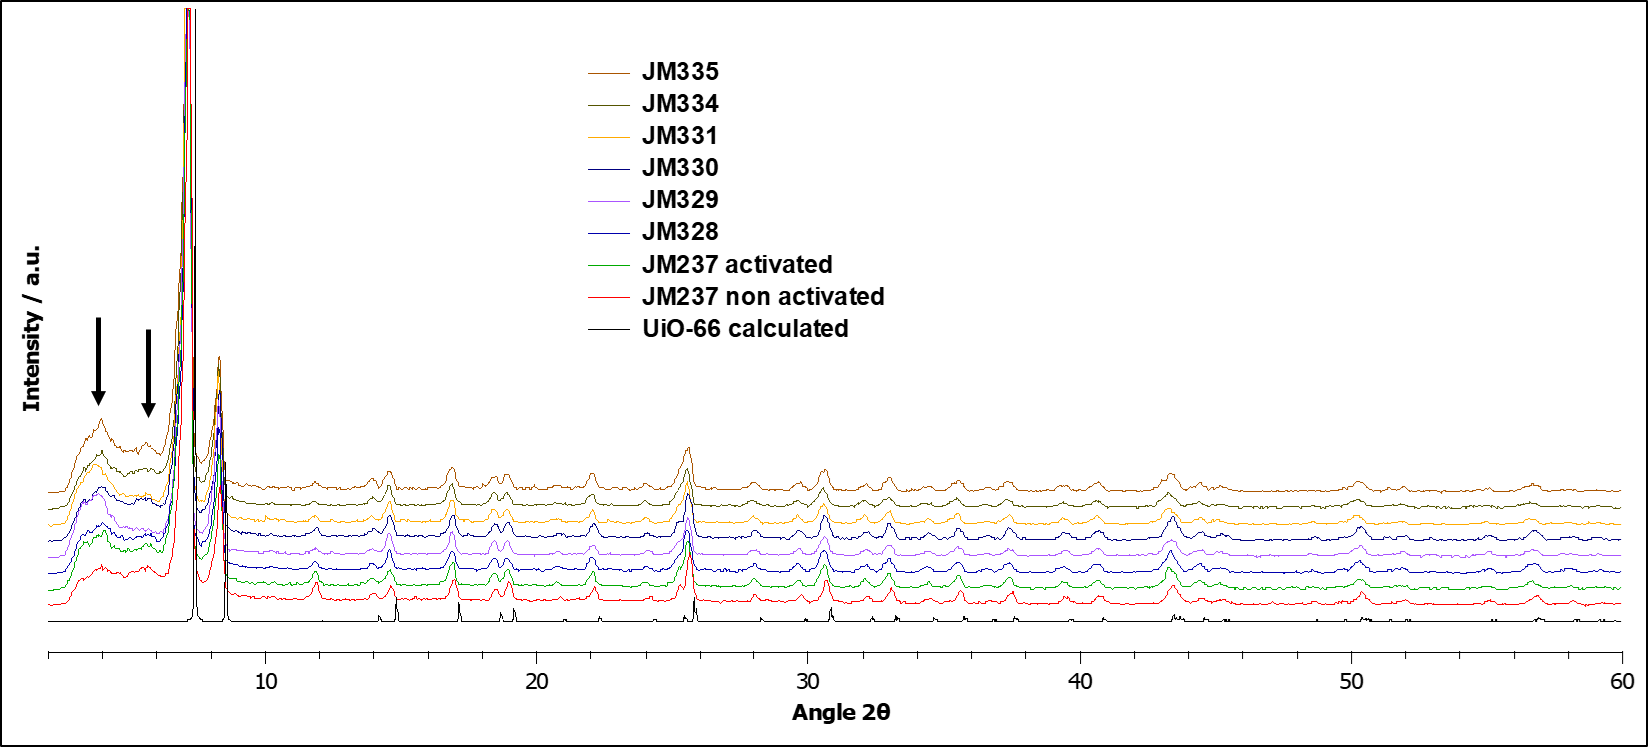
\includegraphics[width=0.6\textwidth]{xrd/xrd-h2o}

    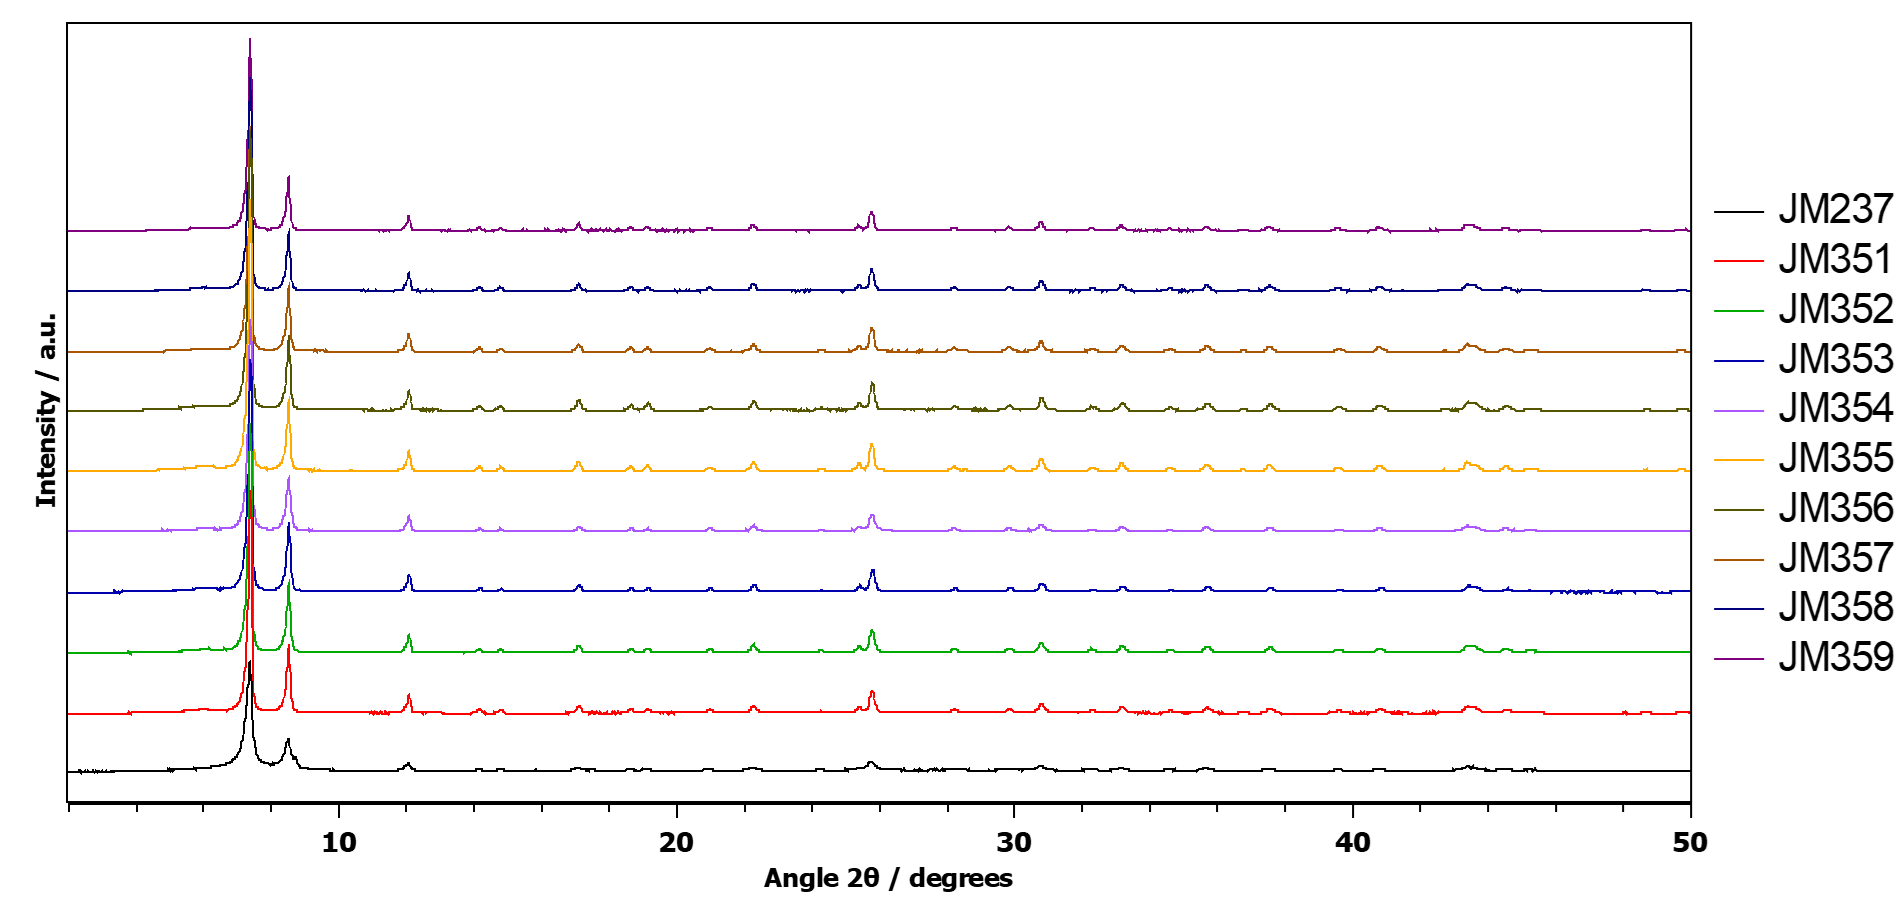
\includegraphics[width=0.6\textwidth]{xrd/xrd-meoh}

    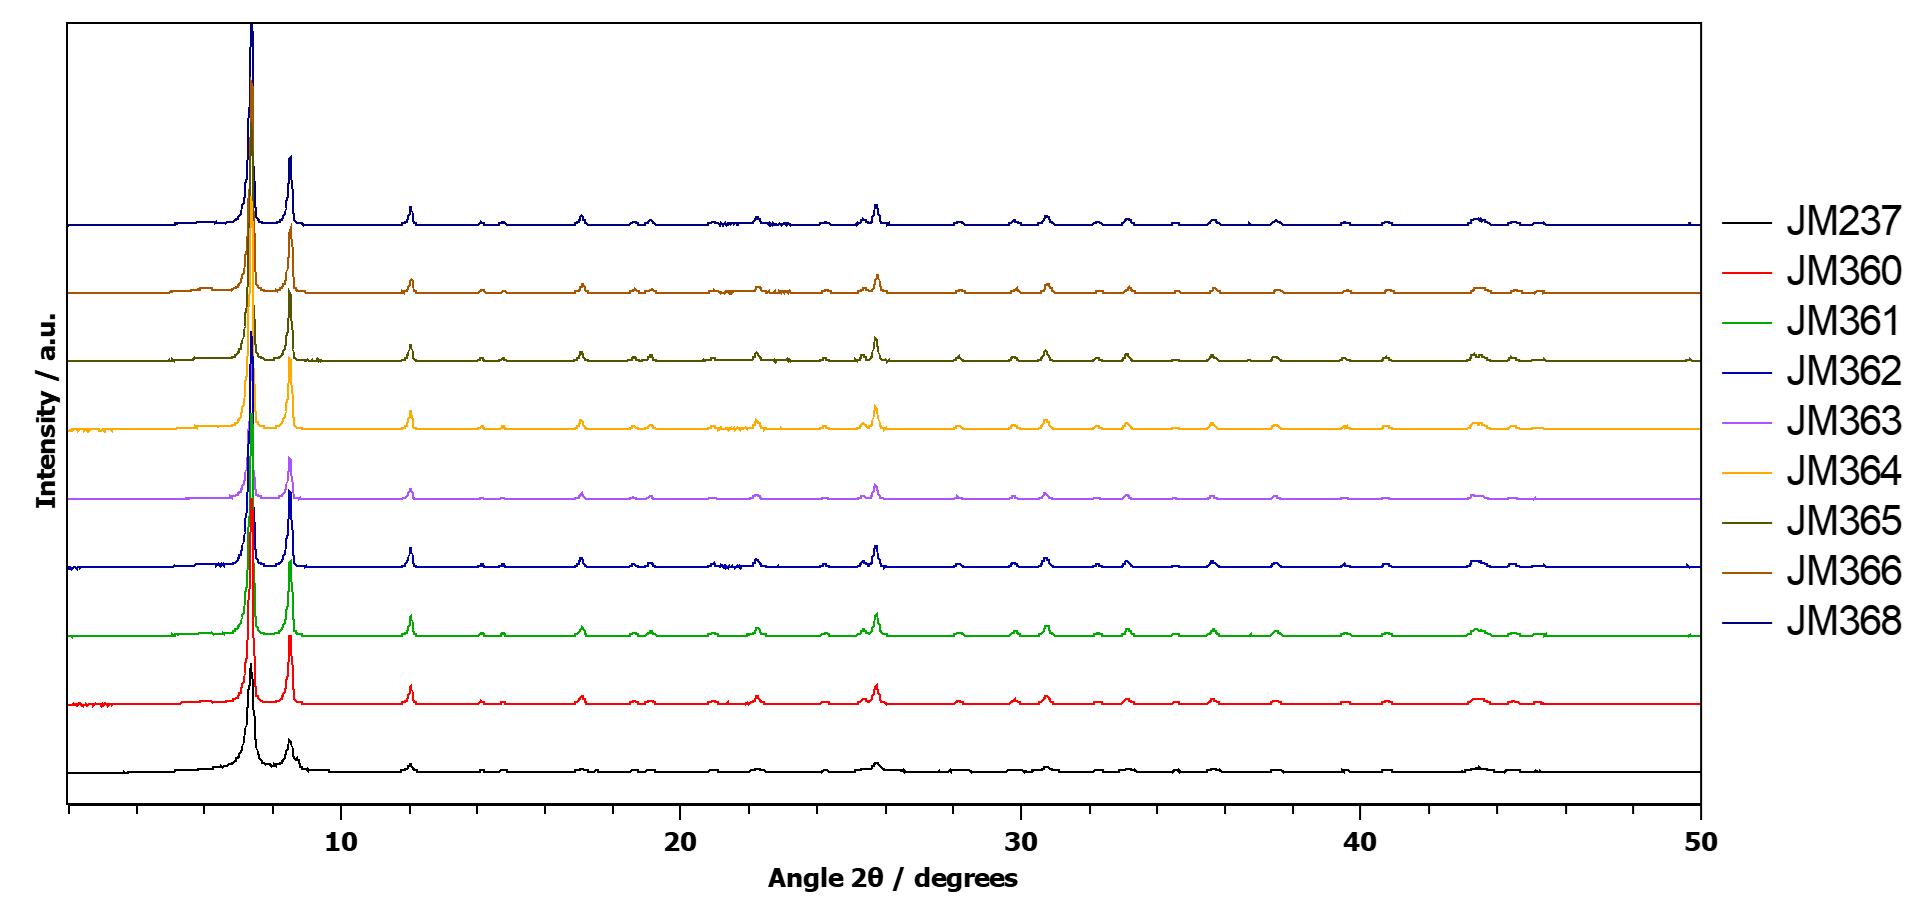
\includegraphics[width=0.6\textwidth]{xrd/xrd-dmso}

    \caption{PXRD patterns for all samples}%
    \label{appx:def:fgr:xrd}
\end{figure}